\documentclass{beamer}
\usetheme{Singapore}
\usepackage[round,sort]{natbib}
\usepackage{tikz}
\usetikzlibrary{arrows,decorations.pathmorphing,backgrounds,fit,positioning,shapes.symbols,chains}
\usepackage{adjustbox}

\title{Structural Contingency Theory}
\subtitle{A Review of Readings}
\author{Ashwin Iyenggar}
\institute[Indian Institute of Management Bangalore] 
{
  Corporate Strategy and Policy\\
  Indian Institute of Management Bangalore
}
\date{22 September, 2016}
\subject{Review of Structural Contingency Theory}

% \pgfdeclareimage[height=0.5cm]{university-logo}{university-logo-filename}
% \logo{\pgfuseimage{university-logo}}

\AtBeginSubsection[]
{
  \begin{frame}<beamer>{Outline}
    \tableofcontents[currentsection,currentsubsection]
  \end{frame}
}

\begin{document}

\begin{frame}
  \titlepage
\end{frame}

\begin{frame}{Outline}
  \tableofcontents
  % You might wish to add the option [pausesections]
\end{frame}

\section{Premise of the Theory}
\subsection{Definitions}

\begin{frame}{Structural Contingency Theory}{Positivist-Functionist}
 \begin{quotation}
"The theory is scientific in style with the aim being to produce scientific knowledge of the type achieved in the natural sciences" \\
\null\hfill \textit{\cite{Donaldson1996a}, on Structural Contingency Theory}
 \end{quotation}
\end{frame}

\begin{frame}{Structural Contingency Theory}{Definition}
Given:
  \begin{itemize}
  \item {
    Environment, e
  }
  \item {
    Contingency, c
  }
  \item {
    Structure, s
  }
  \end{itemize}
  Structural Contingency Theory States:
  \begin{center}e $\rightarrow$ c $\rightarrow$ s\end{center} 
  Environmental uncertainty is seen as causing firms to alter their structure due to task uncertainty (technical uncertainty or strategic uncertainty)\\
  Optimal outcome is produced only by the organization structure that fits the contingency \citep{Lawrence1967}

\end{frame}

\begin{frame}{Structural Contingency Theory}{Operationalization}
Types of Contingencies:
  \begin{itemize}
  \item<1-> {Environment \citep{Lawrence1967} }
  \item<2-> {Internal Technology \citep{Woodward1965}}
  \item<3-> {Organization Size \citep{Child1975,Khandwalla1973,Blau1970,Pugh1969}}
  \item<4-> {Strategy \citep{Chandler1962}}
  \end{itemize}
\end{frame}

\begin{frame}{Structural Contingency Theory}{Relationships}
\begin{figure}[h]
\centering
\begin{adjustbox}{width=\textwidth}
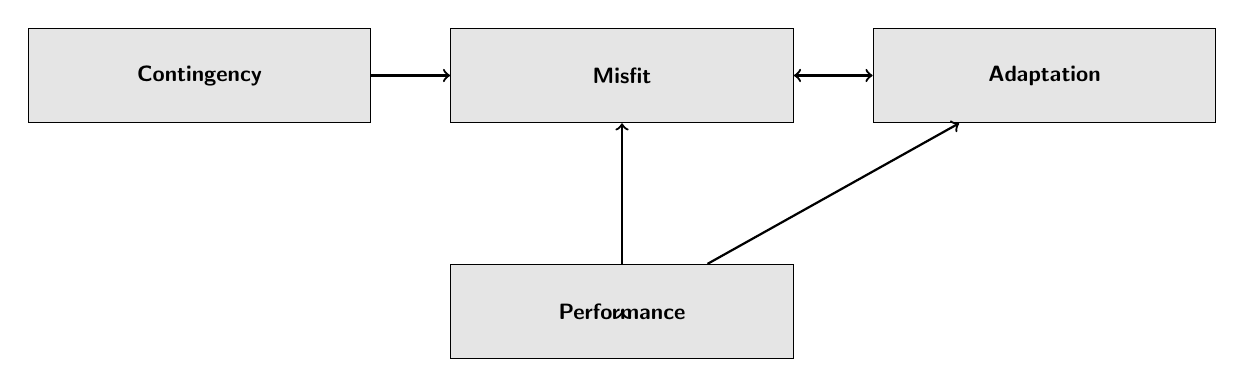
\begin{tikzpicture}
[node distance = 1cm, auto,font=\footnotesize,
every node/.style={node distance=3cm},
comment/.style={rectangle, inner sep= 5pt, text width=4cm, node distance=0.25cm, font=\scriptsize\sffamily},
force/.style={rectangle, draw, fill=black!10, inner sep=5pt, text width=4cm, text badly centered, minimum height=1.2cm, font=\bfseries\footnotesize\sffamily}]

\node [force] (misfit) {Misfit};
\node [force, left=1cm of misfit] (contingency) {Contingency};
\node [force, right=1cm of misfit] (adaptation) {Adaptation};
\node [force, below of=misfit] (performance) {Performance};

\path[->,thick]
(contingency) edge (misfit)
(performance) edge (misfit) edge
(performance) edge (adaptation);

\path[<->,thick]
(misfit) edge (adaptation);

\end{tikzpicture}
\end{adjustbox}
\caption{Relationships in Contingency Theory \citep{Donaldson1987}}
\label{figure:sct}
\end{figure}
\end{frame}


\begin{frame}{Structural Contingency Theory}{Competing Philosophical Underpinnings}

  \begin{itemize}
  \item{Positivist-Functionist }
  \item {Interpretist}
  \item {Conflict}
  \item {Critical}
  \item {Post Modern}
  \end{itemize}
\end{frame}


\subsection{Breaking Away}
\begin{frame}{Breaking Away}{Arrival of New Theories}
  \begin{itemize}
  \item{Population Ecology}
  \item {Institutional Theory}
  \item {Resource Dependence Theory}
  \item {Transaction Cost Economics}
  \end{itemize}
\end{frame}

\begin{frame}{Breaking Away}{Comparison with Economics}
  \begin{itemize}
  \item<1->{Economics \uncover<2->{ - Optimization paradigm offered a coherent theoretical model}}
  \item<3-> {Organization Theory \uncover<4->{ - Structural Contingency Theory was more a program of standardizing empirical research and testing empirical structure-contingency relationships}}
  \item <5->{Reduced strategic task uncertainty in economics}
  \item <6->{Reduced technical task uncertainty in organization theory}
  \end{itemize}
\end{frame}

\section{Points of Debate}

\subsection{Static vs Dynamic}
\begin{frame}{How Dynamic A Theory?}
\begin{itemize}
\item{\cite{Donaldson1987} suggests that the link to performance captures the dynamism required}
\item{\cite{Smith2011} argue that cyclically adjusted response will lead to  short-term peak performance that fuels long term survival}
\item{\cite{Siggelkow2002} suggests that there is path dependence and unintended consequences}
\item{\cite{Miller1992} balances the scales a bit by suggesting that not all choices faced are in conflict}
\item<2->{How dynamic do we need dynamic to be?}
\end{itemize}
\end{frame}

\begin{frame}{Equilibrium vs Process}
\begin{itemize}
\item{\cite{Donaldson1987} assumes that the mechanism from cause to effect is automatic and atomic}
\item{\cite{Siggelkow2002} argues that multiple organizational processes are  possible}
\item<2->{Is the equilibrium model satisfactory in the study of organizations?}
\end{itemize}
\end{frame}

\subsection{Constructs and Assumptions}
\begin{frame}{Constructs: Strict vs Open Ended}
\begin{itemize}
\item{Should the notion of fit be strictly defined?}
\item<2->{Can it be?}
\end{itemize}
\end{frame}

\begin{frame}{Problematic Assumptions}{Notes}
\begin{itemize}
\item{Do organizations  always evolve to higher fit\citep{Payne2006}?}
\item{Does external fit matter more than internal fit?}
\item<2->{How do we deal with disconfirming evidence\citep{Menz2014}?}
\end{itemize}
\end{frame}

\subsection{The Role for Human Agency}

\begin{frame}{The Role for Human Agency}{}
\begin{itemize}
\item{Is the adaptation to fit automatic or driven by managerial intentionality?}
\item<2->{Can managerial intentionality be demonstrated in ways other than toward organizational fit? (Agency Theory, Behavioral Theory)}
\end{itemize}
\end{frame}

\subsection{Time}
\begin{frame}{Time}{}
\begin{itemize}
\item{Contingency has a time invariant, single notion of fit}
\item{\cite{Siggelkow2002} demonstrates that choice between thickening and patching is time variant}
\item{\cite{Smith2011} suggest that firms optimize dual time-horizon objectives}
\item<2->{Should multiple time-period objectives and pressures be included?}
\end{itemize}
\end{frame}

\section{Stepping Back}
\subsection{Assessing the landscape}
\begin{frame}{Perspectives}{}
\begin{itemize}
\item<1->{A strict Positivist-Functionist model is a poor characterization of organizational phenomena}
\item<2->{However, a dominant paradigm that is not falsifiable may be hard to overthrow}
\item<3->{Organization Theory requires its own Dmitri Mendeleev to Organize various Theories in a Coherent Gestalt}
\end{itemize}
\end{frame}

\subsection{A way ahead}
\begin{frame}{Organized in Complex Order}{}
\begin{itemize}
\item<1->{Environment drives Organizational Change, but Organizational Change may also drive Environmental Change}
\item<2->{Simultaneity \citep{Smith2011}}
\item<3->{Influencing role for Internal Agents and External Agents}
\item<4->{Path Dependence and Evolution over Time}
\item<5->{Multiple levels of Analysis}
\end{itemize}
\end{frame}

\begin{frame}{Accuracy vs Parsimony}{}
\begin{itemize}
\item<1->{Computer based models can capture greater complexity than parsimonious theory can}
\item<2->{Should we give up parsimony for accuracy?}
\end{itemize}
\end{frame}

\bibliography{/Users/aiyenggar/OneDrive/code/bibliography/ae,/Users/aiyenggar/OneDrive/code/bibliography/fj,/Users/aiyenggar/OneDrive/code/bibliography/ko,/Users/aiyenggar/OneDrive/code/bibliography/pt,/Users/aiyenggar/OneDrive/code/bibliography/uz}
\bibliographystyle{apalike}

\end{document}
